%!TEX root = ../main.tex

\begin{itemize}
 
  \item 2.1 - describe the jsil language. give its formal syntax  and semantics (extended with assert). 
                   formally define symbolic execution for JSIL commands. soundness result and its corollaries.  
 
  \item 2.2 Implementation:  
               - describe the Rosette approach to the implementation of symbolic analysis 
               - describe the encoding of \jsil concrete/symbolic states in Rosette 
               - explain the \jsil interpreter implemented in Rosette and its connection to the \jsil concrete semantics  and symbolic semantics 
               		- give snippets of the interpreter 
	       		- discuss implementation strategies that enable Rosette to work properly
\end{itemize}

\subsection{Formalisation}

\myparagraph{\jsil: Syntax} \jsil is a goto language featuring top-level procedures and commands operating on object heaps. It was purposefully designed to natively support the main dynamic features of JavaScript: extensible objects; dynamic property access; and dynamic procedure calls. 

%\pg{When talking about JSIL Logic, how are you going to explain the difficulty associated with a dynamci goto language v a static one, I don't think your work is a boring adaptation of reasoning about a staitc goto language. You need to grab at some of this is you can. We've have not paid ebough attention on this, so people jsut think this is a variant of previous work..} 
 
\begin{display}{Syntax of the \jsil Language}\label{def:jsil-types}
\begin{minipage}{\textwidth}
\begin{tabular}{lllll}
	 Numbers: $\jnumber \in \numbers$ & \quad Booleans: $\jbool \in \bools$ & \quad \ Strings: $\jstring \in \strings$ & \quad \ Locs: $\loc \in \locs$ & \quad Vars: $\jvar \in \jvars$ \\[0.1cm]
	Types: $\ivltype \in \ivltypes$ & \multicolumn{4}{l}{\quad Values: $\val \in \vals$ \defeq \ $\jnumber \mid \jbool \mid \jstring \mid  \jsundefined \mid \jsnull \mid \loc \mid \ivltype \mid \fid \mid \jsilempty$} \\[0.1cm]
\multicolumn{5}{l}{Expressions: $\jsilexpr \in \exprs$ \defeq \ $\val \mid \jvar \mid \ominus\ \jsilexpr \mid \jsilexpr \binop{} \jsilexpr $} \\[0.1cm]
	\multicolumn{5}{l}{Basic Commands: $\bcmd \in \bcmds$ \defeq\ $\jsilskip \mid \jvar := \jsilexpr  \mid \jvar := \jsilnew() \mid \jvar := [\jsilexpr, \jsilexpr] \mid [\jsilexpr, \jsilexpr] := \jsilexpr \mid$} \\[0.1cm]
	\multicolumn{5}{l}{\hspace{1.35cm} $\jsildelete(\jsilexpr, \jsilexpr) \mid \jvar := \hasfield(\jsilexpr, \jsilexpr) \mid \jvar := \getfields(\jsilexpr) \mid \assume(\jsilexpr) \mid \assert(\jsilexpr)$} \\[0.1cm]
	% Commands
	\multicolumn{5}{l}{Commands: $\ivlcmd \in \cmds$ \defeq \ $ \bcmd \mid \goto \ i \mid  \ifgoto{\jsilexpr}{i}{j} \mid \jsilcall{\jvar}{\jsilexpr}{\jvec{\jsilexpr}}{j}$} 
 \end{tabular} \\[0.1cm]
 \begin{tabular}{rcrclcl}
 	Procedures & : & $\proc$ & $\in$ & $\procset$ &\defeq& $\procedure{\fid}{\jvec{\jvar}}{\jvec{\ivlcmd}}$ \\[0.1cm]
	%Notation & : & \multicolumn{5}{l}{$\jvec{\jvar}$,  $\jlist{\val}$,  $\overline{\jsilexpr}$, and $\overline{\ivlcmd}$, respectively, denote lists of variables, literals, expressions, and commands. } && \multicolumn{5}{l}{$\set{\val}$ denotes a set of literals.}
 \end{tabular}
 \end{minipage}
 \end{display}
 
%Most syntactic constructs of JSIL either come directly from JavaScript or are useful for JavaScript analysis. 
\jsil values, $\val \in \vals$, include numbers, booleans, strings, the special values $\jsundefined$ and $\jsnull$, as well as types~$\ivltype$, procedure identifiers $\fid$, and the special value $\jsilempty$. 
\jsil~expressions, $\jsilexpr \in \exprs$, include \jsil values, \jsil program variables $\jvar$, and various unary and binary operators, which, for instance, provide support for sets and lists. 



Basic \jsil commands enable the management of extensible objects and do not affect control flow. 
They include $\jsilskip$, variable assignment, object creation, property access, property assignment, property deletion, membership check, property collection, and two special commands, $\assume$ and $\assert$, essential for symbolic execution, but with trivial concrete semantics.

\jsil commands include basic \jsil commands and several commands related to control flow: conditional gotos, unconditional gotos and dynamic procedure calls.\footnote{\jsil also has $\phi$-node commands, which allow the \JSComp compiler to produce code directly in Static-Single-Assignment (SSA) \cite{SSA}. To avoid clutter, we omit the $\phi$-nodes from this formalisation; they do not impact the reasoning in any way. The details can be seen in \cite{javert}.} 
The two goto commands are straightforward: $\goto \ i$ jumps to the $i$-th command of the active procedure, and $\ifgoto{\jsilexpr}{i}{j}$ jumps to the $i$-th command if $\jsilexpr$ evaluates to \jsinline|true|, and to the $j$-th otherwise. 
The dynamic procedure call $\jsilcall{\jvar}{\jsilexpr}{\jvec{\jsilexpr}}{j}$ first evaluates  $\jsilexpr$ and $\jvec{\jsilexpr}$ to obtain the procedure name and arguments, respectively, executes the appropriate procedure with these arguments, and, in the end, assigns its return value to $\jvar$.
If the procedure raises an error, control is transferred to the $j$-th command, and to the next otherwise. 

A \jsil program $\prog \in \ivlprogs$ can be seen as a set of top-level procedures of the form $\procedure{\fid}{\jvec{\jvar}}{\jvec{\jcmd}}$, where $\fid$ is the procedure name, $\jvec{\jvar}$ its formal parameters, and its body ${\jvec{\jcmd}}$  is a \emph{command list} consisting of a numbered sequence of \jsil commands.
Every \jsil program contains a special procedure $\jsilmain$, denoting the entry point of the program. 
\jsil procedures return via two dedicated indexes, $\procretlab$ and $\procerrlab$, using two dedicated variables, $\procretvar$ and $\procerrvar$. If a procedure reaches the $\procretlab$ index, it returns normally with the return value denoted by $\procretvar$; when it reaches $\procerrlab$, it returns an error, with the error value denoted by $\procerrvar$.

\myparagraph{\jsil: Semantics}
The basic memory model of \jsil is as follows. 
%\jsil values contain: numbers, $\jnumber$; booleans, $\jbool$; strings, $\jstring$;  the special values \jsinline|undefined| and \jsinline|null|; and object locations,  $\loc \in \locs$.
A \jsil heap, $\heap \in \heaps$, is a partial function mapping pairs of  object locations, and strings to heap values. 
 Given a heap $\heap$, we denote: a heap cell by $\hcell{\loc}{\jstring}{\val}$, meaning that  $h(\loc,\jstring) = \val$; the union of two disjoint heaps by $\oheap_1 \dunion \oheap_2$; heap lookup by $\hread{\oheap}{\loc}{\jstring}$; and the empty heap by $\hemp$.
 Finally, a \jsil variable store, $\store \in \stores$, is a mapping from JSIL program variables $\jvar \in \jvars$ to JSIL values.

\jsil semantics is defined in small-step style. Transitions for basic commands, given in Figure \ref{fig:sem:basic:commands}, are of the form $\semtrans{\heap, \store, \bcmd}{\heap', \store'}$, meaning that the execution of the basic command $\bcmd$ in the heap $\heap$ and store $\store$ results in the heap $\heap'$ and $\store'$. We also allow a transition of a basic command to fail, denoted by $\semtranserr{\sheap, \sstore, \bcmd}$.

\vspace*{-0.6cm}
\begin{figure}[ht!]
{\scriptsize
\begin{mathpar} 
%
\inferrule[Semantics of expressions]{}{
\semexpr{\val}{\store} \semeq \val
\quad 
\semexpr{\jvar}{\store} \semeq \store(\jvar)
\quad 
\semexpr{\unoper\ \jexpr}{\store} \semeq \unoper (\semexpr{\jexpr}{\store})
\quad 
\semexpr{\jexpr_1 \binoper \jexpr_2}{\store} \semeq \binoper(\semexpr{\jexpr_1}{\store}, \semexpr{\jexpr_2}{\store})}
\\

\inferrule[\textsc{Skip}]{}
	{ \semtrans{\heap, \store, \jsilskip}{\heap, \store}} 
 \qquad
 %
\inferrule[\textsc{Assignment}]
  {
      \symbeval{\jsilexpr}{\store} =  \val
      \quad
      \store' = \store[\jvar \mapsto \val]
  }{\semtrans{\heap, \store, \jvar := \jsilexpr}{\heap, \store'}} 
%
\qquad 
%
\inferrule[\textsc{Object Creation}]
  { 
    \heap = \heap \dunion \hcell{\loc}{\protop}{\jsnull}
    \quad (\loc,-) \notin \domain (\heap)
  }{\semtrans{\heap, \store, \jvar := \jsilnew()}{\heap, \store[\jvar \mapsto \loc]}}
\\
%
\inferrule[\textsc{Property Access}]
  { 
 	\symbeval{\jsilexpr_1}{\store} =  \loc
  	\quad 
        \symbeval{\jsilexpr_2}{\store} =  \jstring
        \quad
        \heap = - \dunion \hcell{\loc}{\jstring}{\val}
  }{ \semtrans{\heap, \store, \jvar := [\jsilexpr_1, \jsilexpr_2]}{\heap,  \store[\jvar \mapsto \val]}}
 \and 
 \inferrule[\textsc{Property Deletion}]
  { 
        \symbeval{\jsilexpr_1}{\store} =  \loc
  	\quad 
        \symbeval{\jsilexpr_2}{\store} =  \jstring
        \quad
        \heap = \heap' \dunion \hcell{\loc}{\jstring}{-}
  }{\semtrans{\heap, \store, \jsildelete(\jsilexpr_1, \jsilexpr_2)}{\heap', \store}}
 %
\\
%
\inferrule[\textsc{Property Assignment - Found}]
  {     \symbeval{\jsilexpr_1}{\store} =  \loc
  	\quad 
        \symbeval{\jsilexpr_2}{\store} =  \jstring
        \quad
        \symbeval{\jsilexpr_3}{\store} =  \val
       \\\\
        \heap = \heap' \dunion  \hcell{\loc}{\jstring}{-}
  }{\semtrans{\heap, \store, [\jsilexpr_1, \jsilexpr_2] := \jsilexpr_3}{\heap' \dunion  \hcell{\loc}{\jstring}{\val}, \store}} 
 \and 
 \inferrule[\textsc{Property Assignment - Not Found}]
  {     \symbeval{\jsilexpr_1}{\store} =  \loc
  	\quad 
        \symbeval{\jsilexpr_2}{\store} =  \jstring
        \quad
        \symbeval{\jsilexpr_3}{\store} =  \val
       \\\\
        \heap = \heap' 
        \quad 
        (\loc, \jstring) \not\in \domain(\heap)
  }{\semtrans{\heap, \store, [\jsilexpr_1, \jsilexpr_2] := \jsilexpr_3}{\heap \dunion  \hcell{\loc}{\jstring}{\val}, \store}} 
\\
%
\inferrule[\textsc{Member Check - True}]
  { 
      \symbeval{\jsilexpr_1}{\store} =  \loc
  	\quad 
        \symbeval{\jsilexpr_2}{\store} =  \jstring
       \quad 
   	(\loc, \jstring) \in \domain(\heap) 
  }{\semtrans{\heap, \store,\jvar := \hasfield(\jsilexpr_1, \jsilexpr_2)}{\heap, \store[\jvar \mapsto \jtrue]}}
  \and 
 \inferrule[\textsc{Member Check - False}]
  { 
      \symbeval{\jsilexpr_1}{\store} =  \loc
  	\quad 
        \symbeval{\jsilexpr_2}{\store} =  \jstring
       \quad 
   	(\loc, \jstring) \not\in \domain(\heap) 
  }{\semtrans{\heap, \store,\jvar := \hasfield(\jsilexpr_1, \jsilexpr_2)}{\heap, \store[\jvar \mapsto \jfalse]}}
%
\\
%
\inferrule[\textsc{Assume}]
  { 
      \symbeval{\jsilexpr}{\store} =  \jtrue
  }{\semtrans{\heap, \store, \assume(\jsilexpr)}{\heap, \store}} 
\and
\inferrule[\textsc{Assert - True}]
  { 
      \symbeval{\jsilexpr}{\store} =  \jtrue
  }{\semtrans{\heap, \store, \assert(\jsilexpr)}{\heap, \store}} 
\and
\inferrule[\textsc{Assert - False}]
  { 
      \symbeval{\jsilexpr}{\store} = \jfalse
  }{\semtranserr{\heap, \store, \assert(\jsilexpr)}} 
\end{mathpar}}
\vspace*{-0.5cm}
\caption{Semantics of \jsil Basic Commands: {$\semtrans{\heap, \store, \bcmd}{\heap', \store'}$}\label{fig:sem:basic:commands}}
\vspace*{-0.5cm}
\end{figure}

To describe transitions for \jsil commands, we introduce call stacks, denoted~$\ctx$. Call stacks are lists of tuples of the form $(\pid, \store, \jvar, i, j)$, where: 
\dtag{1}~$\pid$~is a procedure identifier, 
\dtag{2}~$\store$~is the store of the procedure that called $\pid$, \dtag{3}~$\jvar$~is 
the variable to which the return of $\pid$ must be assigned in $\store$, \dtag{4} $i$ is the index 
of the command to which the control must jump after the execution of $\pid$ in 
case of normal return, and \dtag{5} $j$ the index to which it must jump in case of 
error return. Transitions for control flow commands have the form:  $\semtrans[\prog]{\heap, \store, i}{\heap', \store', i'}[\ctx][\ctx']$, meaning that, in the context of the entire program $\prog$, the evaluation of the $i$-th command of the first procedure in the call stack $\ctx$, in
the heap $\heap$ and store $\store$, generates the heap $\heap'$, store $\store'$, call stack $\ctx'$,   
and the next command to be evaluated is the $i'$-th command of the first procedure of the call stack~$\ctx'$. Due to space constraints and as the transitions for JSIL symbolic execution are  similar, we give the full semantics for JSIL control flow commands in the Appendix. 
% So far, so boring.

\myparagraph{\jsil: Symbolic Semantics}
In order to symbolically execute \jsil programs, we extend the syntax of \jsil expressions with 
symbolic strings $\sstring \in \sstrings$ and symbolic numbers $\snumber \in \snumbers$. 
For convenience, we use $\svars$ to denote the union of $\sstrings$ and $\snumbers$ 
and $\svar$ to range over $\svars$. 

We extend heaps, stores, and call stacks with symbolic values, obtaining symbolic 
heaps, stores, and call stacks, respectively ranged over by $\sheap$, $\sstore$, and $\sctx$. 
A symbolic heap, $\sheap \in \sheaps$, is a partial function mapping pairs of  
object locations, and symbolic expressions to symbolic expressions. 
A symbolic store, $\sstore \in \sstores$, is a mapping from program variables 
$\jvar \in \jvars$ to symbolic expressions.
A symbolic call stack $\sctx$ differs from a concrete call stack in that it contains 
symbolic stores instead of concrete stores.
%
Symbolic expressions $\sexpr \in \sexprs$ are \jsil expressions that do not contain 
any program variables. Put formally, the syntax of symbolic expressions is as follows: 
$\sexpr \triangleq \val \mid \sstring \mid \snumber \mid \unoper\ \sexpr \mid \sexpr \binoper \sexpr$.
The symbolic evaluation of a \jsil expression $\jsilexpr$ in a symbolic store $\sstore$ yields a 
symbolic expression $\sexpr$. Below, we show the rules for evaluating a given \jsil expression with 
respect to a given symbolic store. 

\begin{display}{Symbolic Semantics of Expressions}
\begin{mathpar}
\inferrule[]{}{\semexpr{\val}{\sstore} \semeq \val}
\and
\inferrule[]{}{\semexpr{\svar}{\sstore} \semeq \svar}
\and 
\inferrule[]
	{\semexpr{\jsilexpr}{\sstore} = \val \quad \val' = \semop{\unoper} \val}
	{\semexpr{\unoper\ \jsilexpr}{\sstore} \semeq \val'}
\and
\inferrule[]
	{\semexpr{\jsilexpr}{\sstore} = \sexpr \not\in \vals}
	{\semexpr{\unoper\ \jsilexpr}{\sstore} \semeq \unoper \ \sexpr}
\and 
\inferrule[]
	{\semexpr{\jsilexpr_1}{\sstore} = \val_1 
	  \quad 
	  \semexpr{\jsilexpr_2}{\sstore} = \val_2
	}
	{\semexpr{\jsilexpr_1 \binoper \jsilexpr_2}{\sstore} \semeq \semop{\binoper}(\val_1, \val_2)}
\and 
\inferrule[]
	{\semexpr{\jsilexpr_1}{\sstore} = \sexpr_1 
	  \quad 
	  \semexpr{\jsilexpr_2}{\sstore} = \sexpr_2
	  \quad 
	  \sexpr_1 \not\in \vals \ \vee \ \sexpr_2 \not\in \vals 
	}
	{\semexpr{\jsilexpr_1 \binoper \jsilexpr_2}{\sstore} \semeq \val_1 \, {\binoper} \, \val_2}
\end{mathpar}
\end{display}


%
A \emph{symbolic state} $\sstate = (\sheap, \sstore, \sctx, \pc)$ is a 4-tuple consisting of a 
symbolic heap $\sheap$, a symbolic store $\sstore$, a symbolic call stack $\sctx$, and a path condition $\pc$. 
The path condition is a first-order quantifier-free formula over symbolic strings and 
numbers, which accumulates constraints on the given symbolic inputs that trigger 
the execution to follow the path that led to the current symbolic state. 
Path conditions are given by the following grammar: 
\begin{equation*}
\pc \triangleq \sexpr_1 = \sexpr_2 \mid \sexpr_1 \leq \sexpr_2 \mid \pc_1 \, \wedge \, \pc_2 \mid \pc_1 \vee \pc_2 \mid \neg \pc \mid \jtrue \mid \jfalse
\end{equation*}

Figure~\ref{fig:symbexe:bcmds} presents the symbolic execution rules for \jsil basic commands. 
Rules have the form $\symbtrans{\sheap, \sstore, \bcmd, \pc}{\sheap', \sstore', \pc'}$, 
where: \dtag{1} $\sheap$ and $\sstore$ are the symbolic heap and store on which to evaluate $\bcmd$, 
\dtag{2} $\pc$ the current \emph{path condition}, and \dtag{3} $\sheap'$, $\sstore'$, and $\pc'$
the resulting symbolic heap, store, and path condition. Notice that the rules are non-deterministic.

Figure~\ref{fig:symbexe:cmds} presents the symbolic execution rules for \jsil commands. 
Rules have the form $\symbtrans[\prog]{\sheap, \sstore, i, \pc}{\sheap', \sstore', i', \pc'}[\sctx][\sctx']$; 
they are analogous to the semantic rules for \jsil commands, except that the heap, store, and call stack are symbolic, there is the additional path condition, and their execution can fail. For clarity, we keep the program and the context implicit wherever possible, and make use of a function $\ccmd{\prog, \ctx, i}$, which returns the $i$-th command of the procedure that is first in $\ctx$. We write $\ccmd{i}$ when $\prog$ and $\ctx$ are implicit.


\begin{wrapfigure}{R}{0.4\textwidth}
\vspace*{-0.7cm}
{\small
\hspace*{0.25cm} $\mathtt{0\quad o := new\ ()}$ \\
\hspace*{0.25cm} $\mathtt{1\quad o[\hat{s}] := 42};$ \\
\hspace*{0.25cm} $\mathtt{2\quad x := getFields(o);}$ \\
\hspace*{0.25cm} $\mathtt{3\quad assert\ (llen \ x == 2)}$
}
\vspace*{-0.5cm}
\end{wrapfigure}
The rules for skip, the assignment, object creation, assume, and assert are straightforward. The remaining rules follow a specific pattern. To get a better intuition of how these rules work, let us take a look at the snippet of code shown on the right. 
This code: 
	0)~creates a new object $\mathtt{o}$;
	1)~assigns 42 to a symbolic property $\mathtt{\hat{s}}$ of $\mathtt{o}$; 
	2)~collects all the properties of $\mathtt{o}$ into a list and assigns this list to $\mathtt{x}$; and
	3)~asserts that the length of the list in $\mathtt{x}$ is 2, i.e.~that~$\mathtt{o}$ has two properties in the end. This last assertion will fail. Let us understand why.

%\begin{display}{}
\begin{figure}[ht!]
{\scriptsize
\begin{mathpar} 
%
\inferrule[\textsc{Skip}]{}
	{ \symbtrans{\sheap, \sstore, \jsilskip, \pc}{\sheap, \sstore, \pc}} 
 \quad
 %
\inferrule[\textsc{Assignment}]
  {
      \symbeval{\jsilexpr}{\sstore} =  \sexpr
      \\\\
      \sstore' = \sstore[\jvar \mapsto \sexpr]
  }{\symbtrans{\sheap, \sstore, \jvar := \jsilexpr, \pc}{\sheap, \sstore', \pc}} 
%
\quad 
%
\inferrule[\textsc{Object Creation}]
  { 
    \sheap' = \sheap \dunion \hcell{\loc}{\protop}{\jsnull}
    \\\\
    \and (\loc,-) \notin \domain (\sheap)
  }{\symbtrans{\sheap, \sstore, \jvar := \jsilnew(), \pc}{\sheap', \sstore[\jvar \mapsto \loc], \pc}}
\\
%
\inferrule[\textsc{Property Access}]
  { 
 	\symbeval{\jsilexpr_1}{\sstore} =  \loc
  	\quad 
        \symbeval{\jsilexpr_2}{\sstore} =  \sexpr_p
        \quad
        \sheap = \sheap' \, \uplus \, \big((l, \sexprp_i) \mapsto \sexprv_i\big)\mid_{i = 0}^n   
        \quad
        (l, -) \not\in \domain(\sheap')
        \quad 
        0 \leq k \leq n
        \\\\
        \pc' = \pc \ \wedge \, \big( (\sexprp_k = \sexpr_p) \ \wedge \bigwedge_{i = 0, i \neq k}^n (\sexprp_i \neq \sexpr_p) \big)
  }{ \symbtrans{\sheap, \sstore, \jvar := [\jsilexpr_1, \jsilexpr_2], \pc}{\sheap,  \sstore[\jvar \mapsto \sexprv_k], \pc'}}
 %
\\
%
\inferrule[\textsc{Property Assignment - Found}]
  {     \symbeval{\jsilexpr_1}{\sstore} =  \loc
  	\quad 
        \symbeval{\jsilexpr_2}{\sstore} =  \sexpr_p
        \quad
        \symbeval{\jsilexpr_3}{\sstore} =  \sexpr_v
       \quad 
        \sheap = \sheap' \, \uplus \, \big((l, \sexprp_i) \mapsto \sexprv_i\big)\mid_{i = 0}^n   
        \quad
        (l, -) \not\in \domain(\sheap')
        \quad 
        0 \leq k \leq n
        \\
          \pc' = \pc \ \wedge \, \big( (\sexprp_k = \sexpr_p) \ \wedge \bigwedge_{i = 0, i \neq k}^n (\sexprp_i \neq \sexpr_p) \big)
         \quad
         \sheap'' = \sheap' \, \uplus \,  \big((l, \sexprp_i) \mapsto \sexprv_i\big)\mid_{i = 0, i \neq k}^n \, \uplus \,  (l, \sexpr_p) \mapsto \sexpr_v
  }{\symbtrans{\sheap, \sstore,  [\jsilexpr_1, \jsilexpr_2] := \jsilexpr_3, \pc}{\sheap'', \sstore, \pc'}} 
\\
%
\inferrule[\textsc{Property Assignment - Not Found}]
  {     \symbeval{\jsilexpr_1}{\sstore} =  \loc
  	\quad 
        \symbeval{\jsilexpr_2}{\sstore} =  \sexpr_p
        \quad
        \symbeval{\jsilexpr_3}{\sstore} =  \sexpr_v
       \quad 
        \sheap = \sheap' \, \uplus \, \big((l, \sexprp_i) \mapsto \sexprv_i\big)\mid_{i = 0}^n   
        \quad
        (l, -) \not\in \domain(\sheap')
        \quad 
        0 \leq k \leq n
        \\
          \pc' = \pc \ \wedge \, \bigwedge_{i = 0}^n (\sexprp_i \neq \sexpr_p)
         \quad
         \sheap'' = \sheap \, \uplus \,  (l, \sexpr_p) \mapsto \sexpr_v
  }{\symbtrans{\sheap, \sstore, [\jsilexpr_1, \jsilexpr_2] := \jsilexpr_3, \pc}{\sheap'', \sstore, \pc'}}   
%
\\
%
\inferrule[\textsc{Property Deletion}]
  { 
        \symbeval{\jsilexpr_1}{\sstore} =  \loc
  	\quad 
        \symbeval{\jsilexpr_2}{\sstore} =  \sexpr_p
       \quad 
        \sheap = \sheap' \, \uplus \, \big((l, \sexprp_i) \mapsto -\big)\mid_{i = 0}^n   
        \quad
        (l, -) \not\in \domain(\sheap')
        \quad 
        0 \leq k \leq n
     \\ 
      \pc' = \pc \ \wedge \, \big( (\sexprp_k = \sexpr_p) \ \wedge \bigwedge_{i = 0, i \neq k}^n (\sexprp_i \neq \sexpr_p) \big)
     \quad 
      \sheap'' = \sheap' \, \uplus \,  \big((l, \sexprp_i) \mapsto \sexprv_i\big)\mid_{i = 0, i \neq k}^n
   }{\symbtrans{\sheap, \sstore, \jsildelete(\jsilexpr_1, \jsilexpr_2), \pc}{\sheap'', \sstore, \pc'}}
 \\
 %
\inferrule[\textsc{Member Check - True}]
  { 
      \symbeval{\jsilexpr_1}{\sstore} =  \loc
  	\quad 
        \symbeval{\jsilexpr_2}{\sstore} =  \sexpr_p
       \quad 
        \sheap = \sheap' \, \uplus \, \big((l, \sexprp_i) \mapsto -\big)\mid_{i = 0}^n   
        \quad
        (l, -) \not\in \domain(\sheap')
        \quad 
        0 \leq k \leq n
     \\ 
     \pc' = \pc \ \wedge \, \big( (\sexprp_k = \sexpr_p) \ \wedge \bigwedge_{i = 0, i \neq k}^n (\sexprp_i \neq \sexpr_p) \big)
  }{\symbtrans{\sheap, \sstore, \jvar := \hasfield(\jsilexpr_1, \jsilexpr_2), \pc}{\sheap, \sstore[\jvar \mapsto \jtrue], \pc'}}
%
\\
%
\inferrule[\textsc{Member Check - False}]
  { 
      \symbeval{\jsilexpr_1}{\sstore} =  \loc
  	\quad 
        \symbeval{\jsilexpr_2}{\sstore} =  \sexpr_p
       \quad 
        \sheap = \sheap' \, \uplus \, \big((l, \sexprp_i) \mapsto -\big)\mid_{i = 0}^n   
        \quad
        (l, -) \not\in \domain(\sheap')
        \quad 
        0 \leq k \leq n
     \\ 
     \pc' = \pc \ \wedge \,  \bigwedge_{i = 0}^n (\sexprp_i \neq \sexpr_p) \big)
  }{\symbtrans{\sheap, \sstore, \jvar := \hasfield(\jsilexpr_1, \jsilexpr_2), \pc}{\sheap, \sstore[\jvar \mapsto \jfalse], \pc'}}
\\
%
\inferrule[\textsc{Assert - True}]
  { 
      \symbeval{\jsilexpr}{\sstore} =  \sexpr
     \quad 
     \pc \vdash \sexpr 
  }{\symbtrans{\sheap, \sstore, \assert(\jsilexpr), \pc}{\sheap, \sstore, \pc}} 
\quad
\inferrule[\textsc{Assert - False}]
  { 
      \symbeval{\jsilexpr}{\sstore} =  \sexpr
     \quad 
     \pc \vdash \neg\sexpr 
  }{\symbtranserr{\sheap, \sstore, \assert(\jsilexpr), \pc}{}{\pc}}
  \quad
%
\inferrule[\textsc{Assume}]
  { 
      \symbeval{\jsilexpr}{\sstore} =  \sexpr
     \quad 
     \pc \vdash \sexpr 
  }{\symbtrans{\sheap, \sstore, \assume(\jsilexpr), \pc}{\sheap, \sstore, \pc \land \sexpr}} 
\end{mathpar}}
\vspace*{-0.6cm}
\caption{Symbolic Execution for \jsil Basic Commands: {$\symbtrans{\sheap, \sstore, \bcmd, \pc}{\sheap', \sstore', \pc'}$}\label{fig:symbexe:bcmds}}
\end{figure}
%\end{display}  


\begin{figure}[ht]
{\scriptsize
\begin{mathpar} 
\inferrule[\textsc{Basic Command}]
   { 
     \ccmd{i} = \bcmd 
     \quad
     \symbtrans{\sheap, \sstore, \bcmd, \pc}{\sheap', \sstore', \pc'} 
   }{\symbtrans{\sheap, \sstore, i, \pc}{\sheap', \sstore', i+1, \pc'}}
%
   \qquad
  %
  \inferrule[\textsc{Basic Command - Fail}]
   { 
     \ccmd{i} = \bcmd 
     \quad
     \symbtranserr{\sheap, \sstore, \bcmd, \pc}{}{\pc}
   }{\symbtranserr{\sheap, \sstore, i, \pc}{}{\pc}}
 %
   \qquad
  %
  \inferrule[\textsc{Goto}]
   { \ccmd{i} = \goto \, j \quad}
   {\symbtrans{\sheap, \sstore, i, \pc}{\sheap, \sstore, j, \pc}}
  \\ 
  \inferrule[\textsc{Cond. Goto - True}]
   { \ccmd{i} =  \ifgoto{\jsilexpr}{j}{k} \quad
     \symbeval{\jsilexpr}{\sstore} =  \sexpr
   }
   {\symbtrans{\sheap, \sstore, i, \pc}{\sheap, \sstore, j,  \pc \, \wedge \, \sexpr}}
  \and 
    \inferrule[\textsc{Cond. Goto - False}]
   { \ccmd{i} =  \ifgoto{\jsilexpr}{j}{k} \quad
     \symbeval{\jsilexpr}{\sstore} =  \sexpr
   }
   {\symbtrans{\sheap, \sstore, i, \pc}{\sheap, \sstore, k, \pc \, \wedge \, \neg\sexpr}}
   \\
    \inferrule[\textsc{Procedure Call}]
   { 
    \ccmd{i} =   \jsilcall{\jvar}{\jsilexpr}{\jsilexpr_i \mid_{i = 0}^{n}}{j}
     \quad
    \symbeval{\jsilexpr}{\sstore} =  \pid' 
    \quad
      \symbeval{\jsilexpr_i}{\sstore} =  \sexpr_i \mid_{i = 0}^{n} 
     \quad
     \args(\pid') = \jsillist{\jvar_1, ..., \jvar_{m}} 
     \quad 
      \sexpr_i = \jsundefined \mid_{i = n+1}^{m}  
   }
   {\symbtrans{\sheap, \sstore, i, \pc}{\sheap, [ \jvar_i \mapsto \sexpr_i \mid_{i = 0}^{m}], 0, \pc}[\sctx][(\pid', \sstore, \jvar, i+1, j)::\sctx]}
    \\ 
  \inferrule[\textsc{Normal Return}]
   {
       \sctx = (-, \sstore', \jvar, i, -) :: \sctx' 
       \quad 
       \sstore(\procretvar) = \sexpr
   }  
   {\symbtrans{\sheap, \sstore, \procretlab, \pc}{\sheap, \sstore'[\jvar \mapsto \sexpr], i, \pc}[\sctx][\sctx']}
   \and 
     \inferrule[\textsc{Error Return}]
   {
       \sctx = (-, \sstore', \jvar, -, j) :: \sctx' 
       \quad 
       \sstore(\procerrvar) = \sexpr
   }  
   {\symbtrans{\sheap, \sstore, \procerrlab, \pc}{\sheap, \sstore'[\jvar \mapsto \sexpr], j, \pc}[\sctx][\sctx']}
 \end{mathpar}}
 \vspace*{-0.4cm}
\caption{Symbolic Execution for \jsil Commands: {$\symbtrans{\sheap, \sstore, i, \pc}{\sheap', \sstore', j, \pc'}[\sctx][\sctx']$}\label{fig:symbexe:cmds}}
 \vspace*{-0.4cm}
\end{figure}


Without loss of generality, we can assume to start with an empty heap, empty store, and an empty path condition: $\tuple{\hemp, \emptyset, 0, \jtrue}$. After the execution of the first command, $\mathtt{o := new\ ()}$, using the \textsc{Basic Command} and \textsc{Object Creation} rules, we will have the state $\tuple{\{ \mathtt{l_o : \{ ``@proto" : null} \} \}, \{ \mathtt{o : l_o} \} , 1, \jtrue}$, illustrated at the top of the figure below.

%\vspace*{-0.3cm}
\begin{figure*}[h!]
\centering
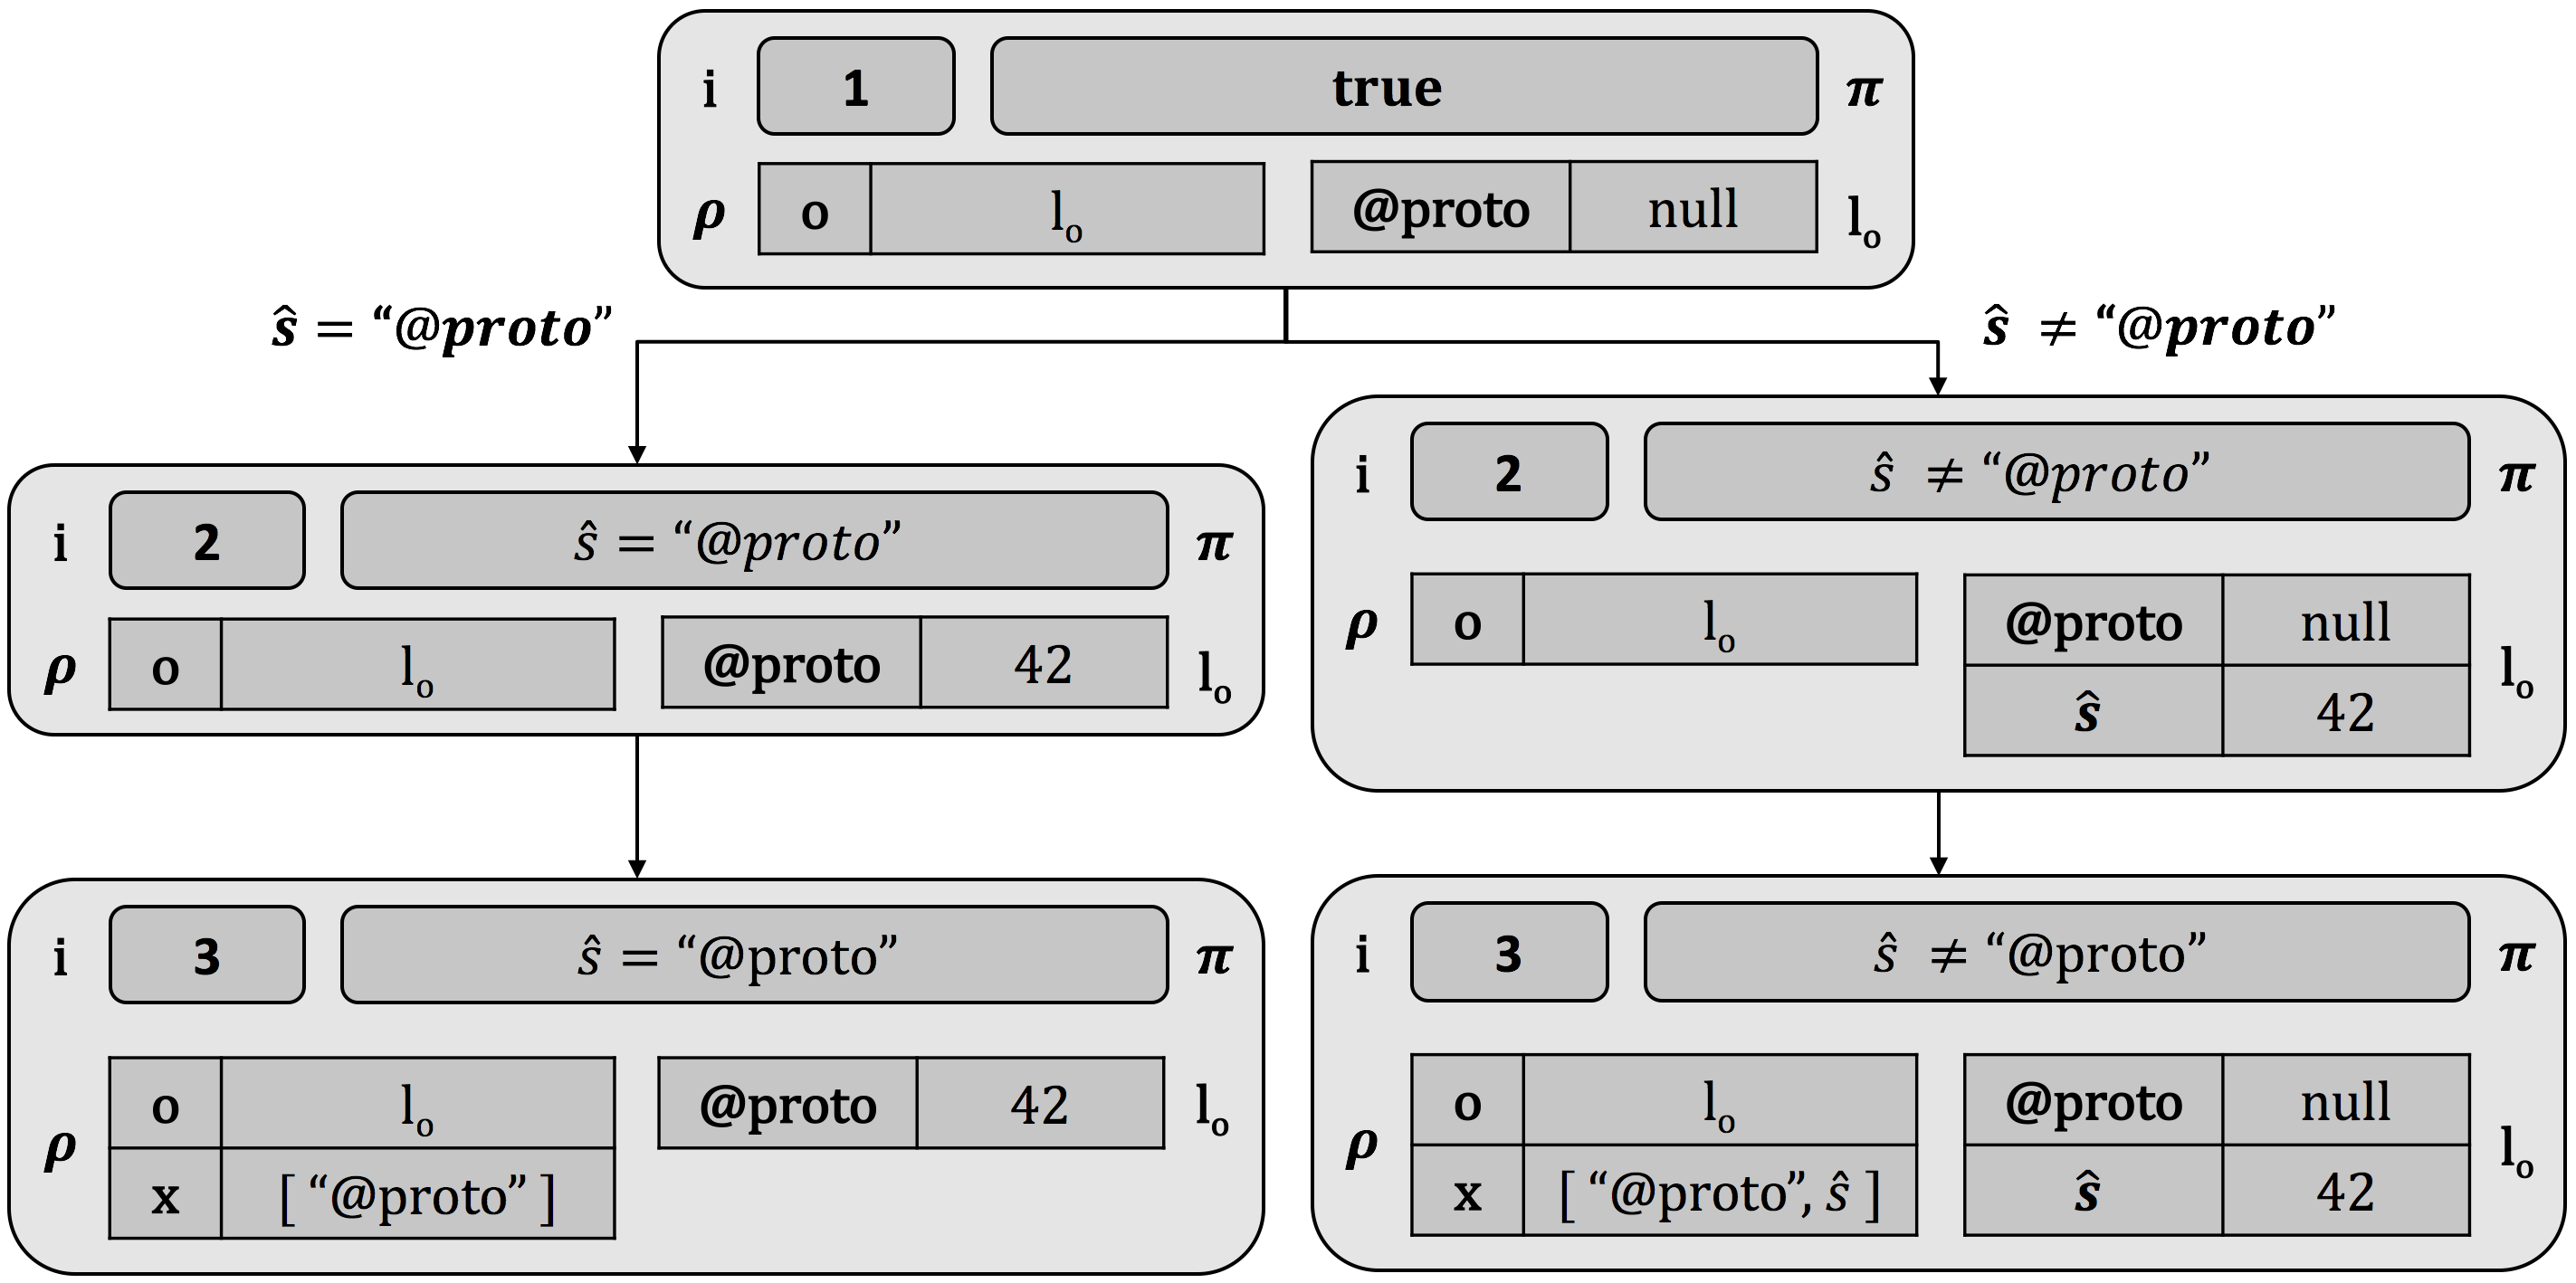
\includegraphics[width=0.83\textwidth]{symbSemEx.png}
%\vspace*{-0.3cm}
\end{figure*}

The next command to be executed is the property assignment $\mathtt{o[\hat{s}] := 42}$. In the semantics, there are two potential \textsc{Property Assignment} rules (\textsc{Found}, \textsc{Not Found}), and in our case, both of them are applicable. The strategy is to non-deterministically allow the targeted property of the object, (in our case, the symbolic property $\hat{s}$ of object $\mathtt{l_o}$), to be equal to any of the already existing properties of the object (in our case, we have only $\mathtt{``@proto"}$), and also allow it to be different from them all, adding the appropriate condition to the path condition, and proceeding to the next command. \polish{I stopped here.}




$\symbeval{\jsilexpr_1}{\sstore} = \mathtt{l_o}$, $\symbeval{\jsilexpr_2}{\sstore} = \hat{s}$, and $\symbeval{\jsilexpr_3}{\sstore} = 42$. We also have that $\sheap' = \hemp$, $n = 0$, $\sexprp_0 = \mathtt{``proto"}$, and $\sexprv_0 = \jsnull$.   









\myparagraph{Soundness} To establish the soundness of symbolic execution, we need to relate 
symbolic states to concrete states. To this end, we make use of \emph{symbolic environments} 
$\senv : \svars \rightharpoonup \vals$ mapping symbolic values to concrete values. 
A symbolic environment is said to be \emph{well-formed} if it maps symbolic 
values to concrete values of the appropriate type (e.g. symbolic strings are mapped to strings 
and symbolic numbers are mapped to numbers). In the following, we will always 
assume well-formed symbolic environments. 
%
Given a symbolic environment $\senv$, we define the interpretation of symbolic 
expressions, heaps, stores, and contexts as shown in Figure~\ref{fig:symbolic:interp}. 
We say that a symbolic environment is \emph{consistent} with a path condition 
$\pc$, written $\senv \vdash \pc$,  if and only if $\semexpr{\pc}{\senv} = \jtrue$. 
Given a symbolic state $(\sheap, \sstore, \sctx)$ and a path condition $\pc$, we define 
the models of the symbolic state under $\pc$, written $\smodels{\sheap, \sstore, \sctx}{\pc}$, 
as the set of concrete states that can be obtained from $(\sheap, \sstore, \sctx)$ using 
logical environments that are consistent with $\pc$. Formally:
\begin{equation}
\smodels{\sheap, \sstore, \sctx}{\pc} = \left\{ (\heap, \store, \ctx) \mid \exists \senv \, . \,  \semexpr{(\sheap, \sstore, \sctx)}{\senv} = (\heap, \store, \ctx) \, \wedge \,  \senv \vdash \pc  \right\} 
\end{equation}

\begin{figure}[!h]
{
\begin{tabular}{l}
$\quad${\bf Interpretation of Symbolic Expressions:}  \\
$
\quad
\semexpr{\val}{\senv} \semeq \val
\quad 
\semexpr{\svar}{\senv} \semeq \senv(\svar)
\quad 
\semexpr{\unoper\ \sexpr}{\senv} \semeq \unoper (\semexpr{\sexpr}{\senv})
\quad 
\semexpr{\sexpr_1 \binoper \sexpr_2}{\senv} \semeq \binoper(\semexpr{\sexpr_1}{\senv}, \semexpr{\sexpr_2}{\senv}) 
$
\\[3pt]
$\quad${\bf Symbolic Heaps:}  \\
$
\quad
 \semexpr{\hemp}{\senv} \semeq \hemp
\quad
\semexpr{\hcell{\loc}{\sexpr_p}{\sexpr_v}}{\senv} \semeq  \hcell{\loc}{\semexpr{\sexpr_p}{\senv}}{\semexpr{\sexpr_v}{\senv}}
\quad
\semexpr{\sheap_1 \dunion \sheap_2}{\senv} \semeq  \semexpr{\sheap_1}{\senv} \dunion \semexpr{\sheap_2}{\senv}
$%
%%
%%
\\[3pt]
$\quad${\bf Symbolic Stores:}  
$
 \semexpr{\storeemp}{\senv} \semeq \storeemp
\quad 
 \semexpr{(\jvar: \sexpr) \dunion \sstore}{\senv} \semeq (\jvar: \semexpr{\sexpr}{\senv}) \dunion \semexpr{\sstore}{\senv}
$%
\\[3pt]
$\quad${\bf Symbolic Contexts:}  
$ \semexpr{\lstemp}{\senv} \semeq \lstemp
\quad 
 \semexpr{(\pid, \sstore, \jvar, i, j) \lstcons \sctx}{\senv} \semeq (\pid, \semexpr{\sstore}{\senv}, \jvar, i, j) \lstcons \semexpr{\sctx}{\senv}
$%

\\[3pt]
$\quad${\bf Symbolic States:}  $\semexpr{(\sheap, \sstore, \sctx)}{\senv} \semeq (\semexpr{\sheap}{\senv}, \semexpr{\sstore}{\senv}, \semexpr{\sctx}{\senv})$
\end{tabular}
}
\caption{Interpretation of symbolic expressions, heaps, stores, and contexts.\label{fig:symbolic:interp}}
\end{figure}

The theorem of soundness states that if we have a symbolic trace $\symbtranstrans{\sheap, \sstore, i, \pc}{\sheap', \sstore', i', \pc'}[\sctx][\sctx']$ 


\begin{theorem}[Soundness of the \jsil symbolic execution]\label{teo:soundness:jsil:symb:exe}
$$
\begin{array}{l}
\forall \, \sheap, \sheap', \heap, \sstore, \sstore', \store, i, i', \sctx, \sctx', \ctx, \pc, \pc' \, . \,  \\  
\quad \symbtranstrans{\sheap, \sstore, i, \pc}{\sheap', \sstore', i', \pc'}[\sctx][\sctx'] 
   \ \wedge \ 
      (\heap, \store, \ctx) \in \smodels{\sheap, \sstore, \sctx}{\pc'} \\ \quad \quad
      	 \ \Rightarrow \ \exists (\heap', \store', \ctx') \, . \, 
	 	 \semtranstrans{\heap, \store, i}{\heap', \store', i'}[\ctx][\ctx']
		\, \wedge \, 
		(\heap', \store', \ctx') \in \smodels{\sheap', \sstore', \sctx'}{\pc'}  
\end{array}
$$
\end{theorem}

\begin{corollary}[Bug Finding]\label{bug:finding}
$$
\begin{array}{l}
\forall \, \sheap, \sstore, \sctx, i, \pc, \pc' \, . \,  
 \symbtranstranserr{\sheap, \sstore, i, \pc}{\sctx}{\pc'}  \ \wedge \  \pc' \text{ is satisfiable} \\ 
   \quad \implies 
     \exists \heap, \store, \ctx \, . \, \semtranstranserr{\heap, \store, i}[\ctx]
\end{array}
$$
\end{corollary}

\begin{corollary}[Verification]\label{corollary:verification}
$$
\begin{array}{l}
\forall \, \sheap, \sheap_1, ..., \sheap_k, \sstore, \sstore_1, ..., \sstore_k, \sctx, \sctx_1, ..., \sctx_k, i, j_1, ..., j_k, \pc, \pc_1, ..., \pc_k \, . \,  \\
  \quad \symbtranstrans{\sheap, \sstore, i, \pc}{\sheap_k, \sstore_k, j_k, \pc_k}[\sctx][\sctx_k]\mid_{k = 1}^n
      \ \wedge \ \pc \vdash \bigvee_{k=1}^n \pc_k \\ 
      \quad \quad \implies 
         \forall \heap, \store, \ctx \, . \, (\heap, \store, \ctx) \in \smodels{\sheap, \sstore, \sctx}{\pc} \\
          \quad \qquad \implies \exists \heap', \store', \ctx' \, . \, 
                  \semtranstrans{\heap, \store, i}{\heap', \store', j_k}[\ctx][\ctx'] \ \wedge \ 
                  (\heap', \store', \ctx') \in \smodels{\sheap_k, \sstore_k, \sctx_k}{\pc_k}
\end{array}   
$$ 
\end{corollary}



\subsection{Implementation}

\polish{The point here is to explain how writing a correct concrete \jsil interpreter in Rosette
yields the symbolic environments presented in the previous subsection.} 

Ideally I would like to talk about: 
\begin{itemize}
   \item how do we represent the \jsil state in Rosette? why did we choose this representation? 
   \item how do we represent \jsil programs as s-expressions? 
   \item ...
\end{itemize}

\begin{display}{Rosette implementation of \jsil symbolic state}
{\scriptsize
\begin{mathpar}
\inferrule[\textsc{Empty Heap}]
  {}{\roscomp{\hemp} \semeq (\racketlist)} 
\and 
\inferrule[\textsc{Non-empty Heap}]
  {
  	 \sheap_1 = \big((l, \sexprp_i) \mapsto \sexprv_i\big)\mid_{i = 0}^n   
	 \quad 
	 (\loc, -) \not\in \domain(\sheap_2)
  }{\roscomp{\sheap_1 \dunion \sheap_2} \semeq  (\racketcons (\racketcons \loc \, (\racketlist \, (\racketcons \sexprp_0 \, \sexprv_0) \cdots   (\racketcons \sexprp_n \, \sexprv_n)))  \ \roscomp{\sheap_2})} 
 \\
\inferrule[\textsc{Empty Store}]
  {}{\roscomp{\storeemp} \semeq (\racketlist)} 
\and 
\inferrule[\textsc{Non-Empty Store}]
  {}{\roscomp{(\jvar: \sexpr) \dunion \sstore} \semeq (\racketcons \, (\racketcons \, (\racketquote \jvar) \ \sexpr) \,  \roscomp{\sstore})} 
\\ 
\inferrule[\textsc{Empty Context}]
  {}{\roscomp{\lstemp} \semeq (\racketlist)} 
\quad 
\inferrule[\textsc{Non-Empty Context}]
  {}{\roscomp{(\fid, \sstore, \jvar, i, j) \lstcons \sctx} \semeq  (\racketcons \,  (\racketlist \, (\racketquote \fid) \, \roscomp{\sstore} \, (\racketquote \jvar) \, i \, j) \, \roscomp{\sctx})} 
\end{mathpar}}
\end{display}

\lstset{language=Scheme}

\begin{figure}
\begin{lstlisting}
(define (mutate-prop-val-list prop-val-list prop new-val)
  (cond
    [(null? prop-val-list)
     (list (cons prop new-val))]
    [(equal? (car (car prop-val-list)) prop)
     (cons (cons prop new-val) (cdr prop-val-list))]
    [ else
     (cons (car prop-val-list) (mutate-prop-val-list (cdr prop-val-list) prop new-val))]))

(define (mutate-heap heap loc prop val)
  (define (mutate-heap-pulp h-pulp loc prop val)
    (cond
      [(null? h-pulp)
       (list (cons loc (list (cons prop val))))]
      [(equal? (car (car h-pulp)) loc)
       (cons (cons loc (mutate-prop-val-list (cdr (car h-pulp)) prop val)) (cdr h-pulp))]
      [ else
       (cons (car h-pulp) (mutate-heap-pulp (cdr h-pulp) loc prop val))]))
  (let ((new-heap-pulp (mutate-heap-pulp (unbox heap) loc prop val)))
    (set-box! heap new-heap-pulp)))


(define (run-bcmd bcmd heap store)
  (let ((cmd-type (first bcmd)))
    (cond
    	[(eq? cmd-type 'h-assign)
      	 (let* ((loc-val (run-expr (second bcmd) store))
                (prop-val (run-expr (third bcmd) store))
                (rhs-val (run-expr  (fourth bcmd) store)))
            (mutate-heap heap loc-val prop-val rhs-val)
            rhs-val)]
         ...)))
\end{lstlisting}
\caption{Fragment of \jsil Interpreter in Rosette}
\end{figure}


\section{Symbolic Execution for JavaScript}

\begin{itemize}
   \item 2.0 Intro - Initial bla bla - the diagram 
   \item 2.1 Symbolic execution for JavaScript 
              - Extending ES5 Strict with asserts, assumes, and symbolic values
              - Extending JS2JSIL with the compilation of the new constructs 
              - Extensible Interpreter 
                   - an easy way to have more coverage 
                   - match the abstraction level of the generated code to the abstraction level of Rosette 
    \item 2.2 - the example 
\end{itemize}

\begin{figure}[t]
\centering
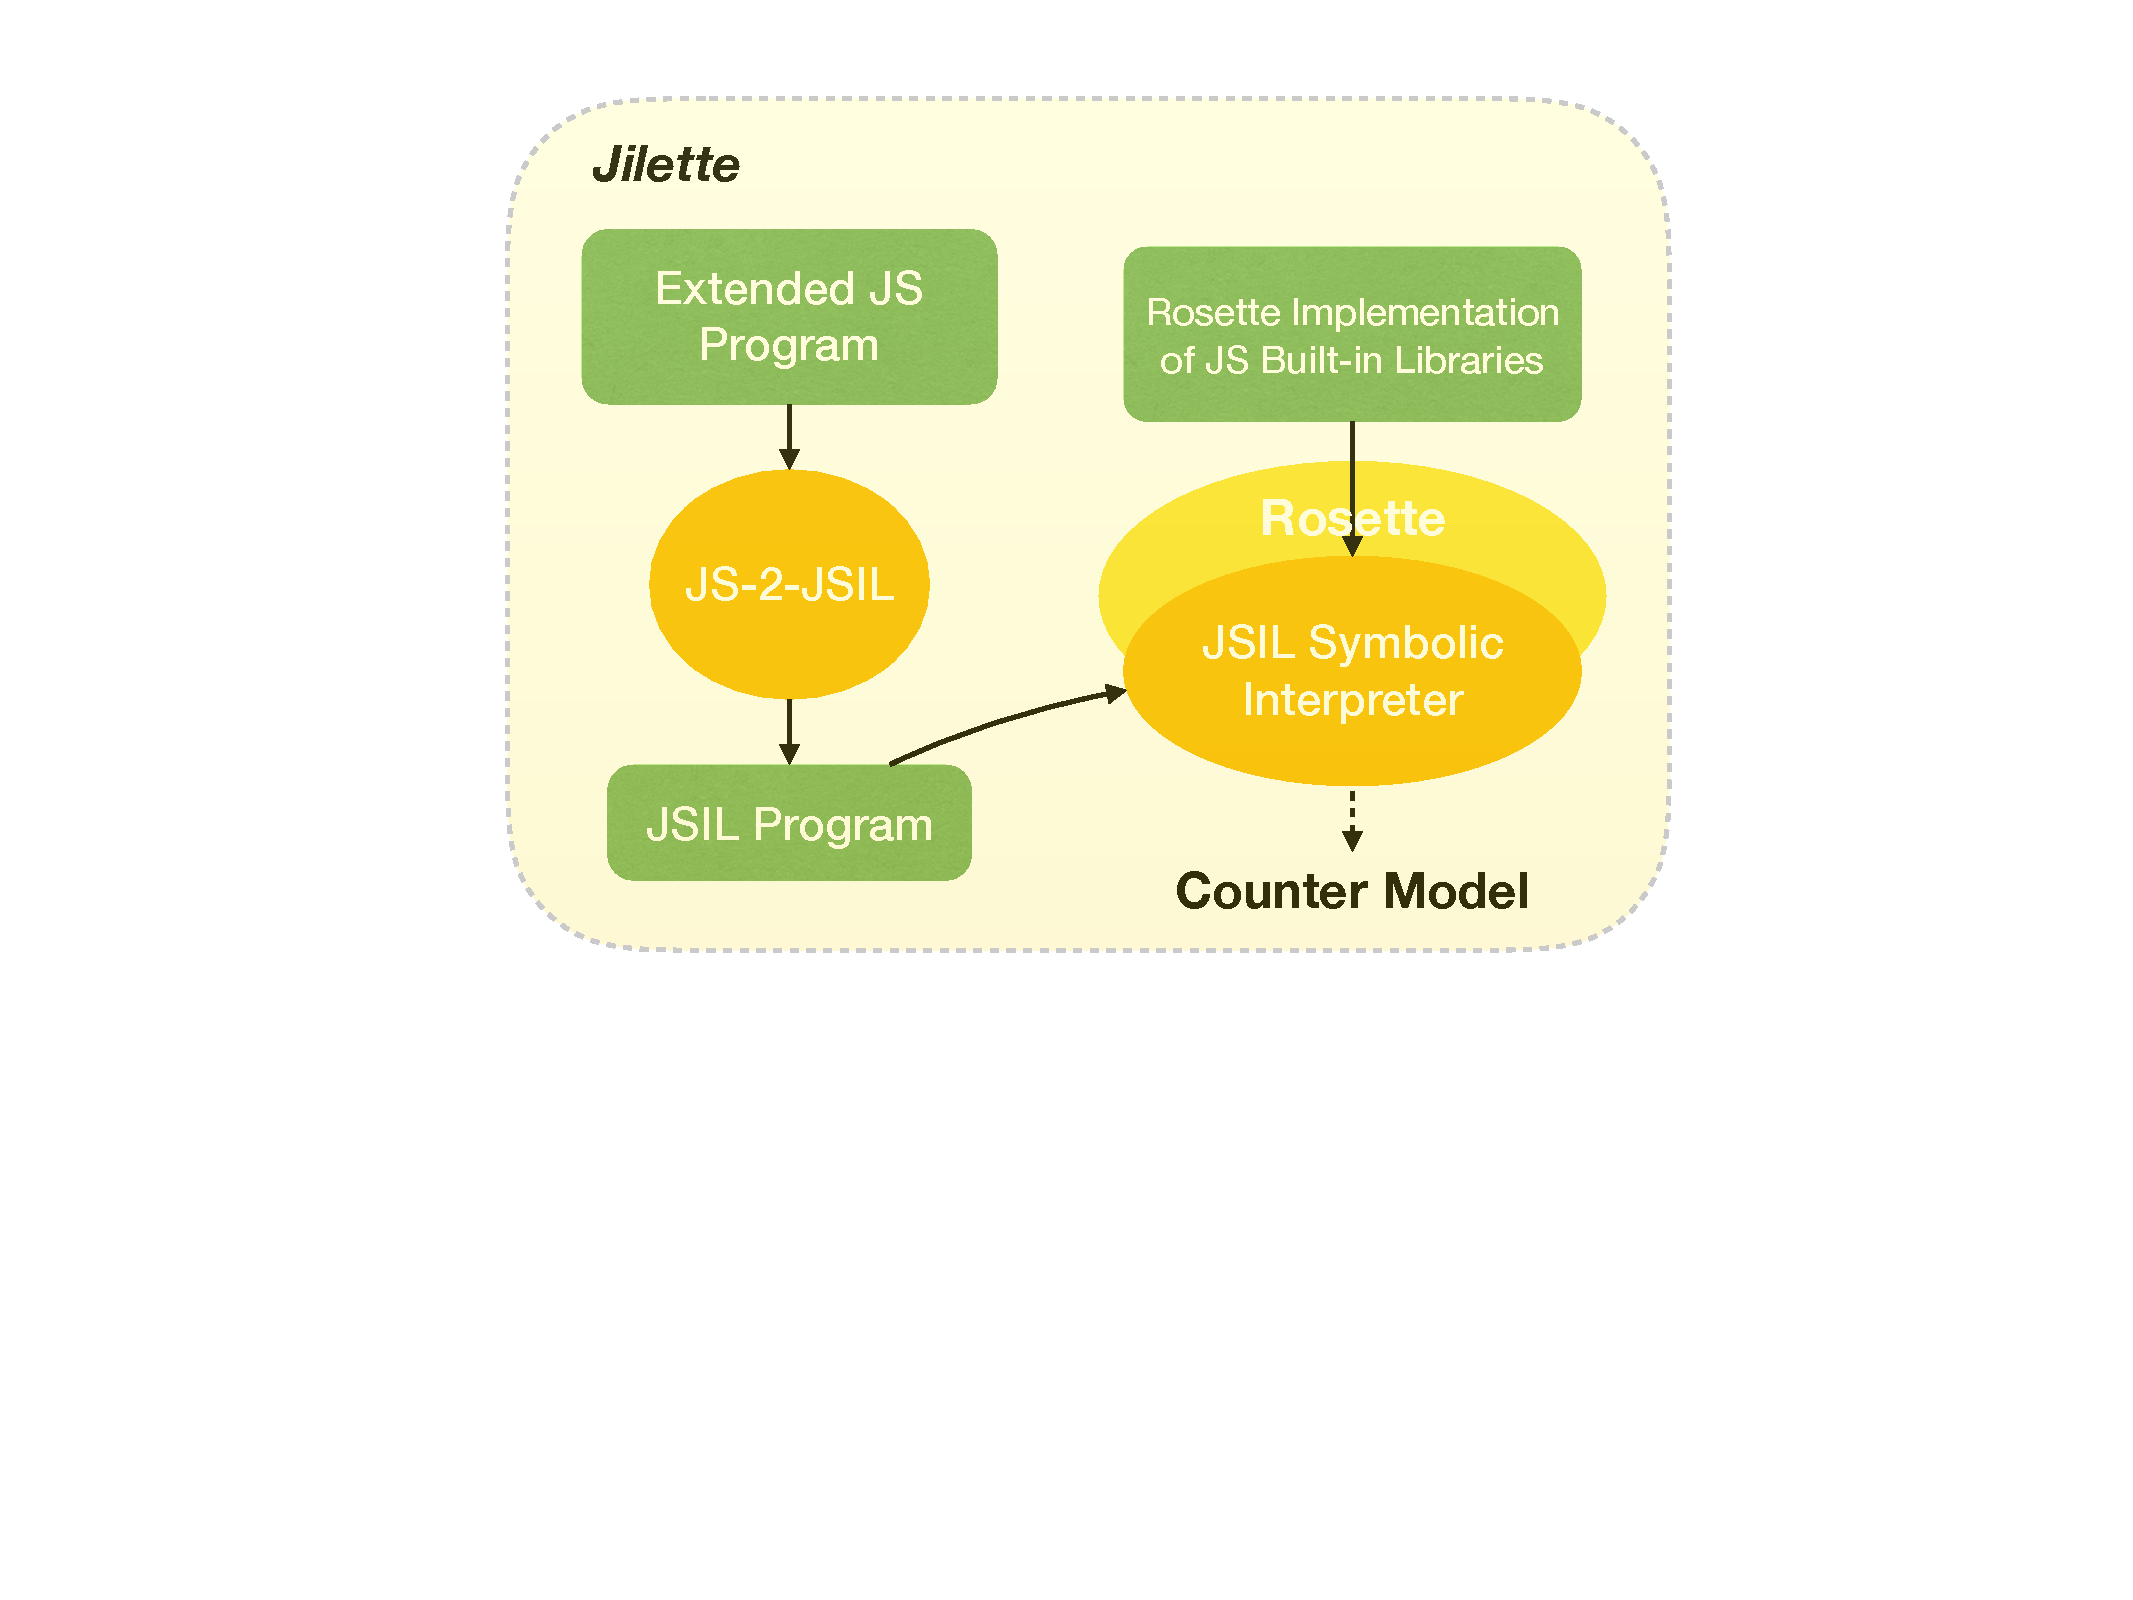
\includegraphics[width=0.7\textwidth]{figures/jilette.pdf}
\caption{Jilette: Symbolic execution for JavaScript}
\label{fig:jilette:diagram}
\end{figure}

The JavaScript standard spans over more than 200 pages describing the language syntax, semantics, 
and runtime environment~\cite{ecma}. The current version of the standard is described in a document with 
more than 800 pages. Clearly, designing a sound symbolic analysis targeting JavaScript directly 
is not the way to go. Besides being error-prone, such a task would require a great amount of engineering effort, 
which would scarcely pay off given the continuous releases of new versions of the standard. 

In order to be able to symbolically execute JavaScript programs, we first extend the language 
with solver-aided facilities for the creation of symbolic values and the checking of assertions. 
For the symbolic execution itself, instead of targeting JavaScript directly, \jilette works by by first 
compiling JavaScript programs to \jsil using the \JSComp compiler.
The obtained \jsil program is then given to the \jsil symbolic interpreter described in \S\ref{sec:jsil:symb:exec}. 
The symbolic interpreter is extensible in that it allows the addition of Rosette implementations of 
JavaScript built-in libraries in a streamlined manner.  
These implementations are both an easy way to get a better coverage of the standard and 
to make sure that we make proper use of the solver-aided facilities of Rosette.    

\subsection{Symbolic Execution by Compilation} 

\myparagraph{Extending JavaScript Syntax}
We extend the syntax of JavaScript with special logical expressions $\jslexpr$, 
and the following constructs: %(corresponding to JavaScript normal expressions): 
\dtag{1} $\jsassert(\jslexpr)$ stating that whenever the \emph{assert} is reached, 
the logical expression $\jslexpr$ must evaluate to $\jtrue$; 
\dtag{2} $\jsassume(\jslexpr)$ stating that we \emph{assume} $\jslexpr$ to hold along the
current program path; 
\dtag{3} $\jssymbstring()$ for creating a fresh symbolic string; and
\dtag{4} $\jssymbnumber()$ for creating a fresh symbolic number. 
The \emph{assert} and \emph{assume} constructs expect as an argument 
a logical expression. 
Logical expressions $\jsexpr$ are given by the grammar 
$\jslexpr \triangleq \jslit \mid \jsvar \mid \unoper\ \jslexpr \mid \jslexpr \binoper \jslexpr$, 
where $\jslit$ ranges over JavaScript literals, $\jsvar$ over JavaScript variables, 
$\unoper$ over the \jsil unary operators, and $\binoper$ over the \jsil binary operators.
It is important to note that JavaScript binary and unary operators have a special 
semantics that most of times includes several implicit type coercions performed
in a specific, and often counter-intuitive, order. 
Hence, instead of allowing for arbitrary JavaScript expressions (using JavaScript 
binary and unary operators) as the arguments for the \emph{assume} and 
the \emph{assert} constructs, we define a simple and restricted syntax for logical expressions.
\polish{The punchline is that the unary and binary operators in the \emph{assume} and 
\emph{assert} constructs are \underline{not} the JavaScript ones but the the \jsil ones with a very clear and 
simple semantics, involving no coercions or side-effects.}

\myparagraph{Extending \JSComp}
Instead of giving a formal semantics for the newly introduced constructs, we explain 
their meaning by showing their compilation to \jsil. 
Importantly, the JavaScript variable store is emulated in the heap. 
Hence, a JavaScript variable $\jsvar$ is not compiled to a \jsil variable $\jvar$, but to a sequence  
of \jsil commands for retrieving the value of $\jsvar$ from the heap cell in which it is stored. 
A full description of the compiler is out of the scope of this paper; c.f.~\cite{javert}
for further details. 
%
In the following, we will assume given a function $\compile : \jstmts \rightharpoonup \lists(\cmds) * \jvars$ mapping JavaScript expressions 
and statements to lists of \jsil commands paired up with \jsil variables. 
In a nutshell, $\compile(\jstmt) = ([ \jcmd_1, ..., \jcmd_n], \jvar)$ means that the compilation 
of the JavaScript statement $\jstmt$ results in the list of \jsil commands $[ \jcmd_1, ..., \jcmd_n]$, 
and that after the execution of these commands, the value to which $\jstmt$ evaluates in the 
JavaScript semantics is stored in the \jsil variable $\jvar$. 
%
Below we show the extension of $\compile$ for the constructs introduced above. 
The definition of $\compile$ makes use of an auxiliary compiler $\compilel : \jlexprs \rightharpoonup \lists(\cmds) * \exprs$, 
for compiling JavaScript logical expressions.

\begin{display}{Extension $\compile : \jstmts \rightharpoonup \lists(\cmds) * \jvars$ and $\compilel : \jlexprs \rightharpoonup \lists(\cmds) * \exprs$}
{\scriptsize
\begin{mathpar}
\inferrule[\textsc{Assume}]
  {
     \compilel(\jslexpr) = [\jcmd_1, ..., \jcmd_n], \jvar
     \and 
     \jvar' \text{ fresh} 
     \\\\ 
     \jcmd_{n+1} = \jvar' := \jsilempty 
     \quad
     \jcmd_{n+2} = \assume(\jvar) 
  }{\compile(\jsassert(\jslexpr)) \semeq [\jcmd_1, ..., \jcmd_n, \jcmd_{n+1}, \jcmd_{n+2}], \jvar'} 
\and
\inferrule[\textsc{Assert}]
  {
     \compilel(\jslexpr) = [\jcmd_1, ..., \jcmd_n], \jvar
     \and 
     \jvar' \text{ fresh} 
     \\\\ 
     \jcmd_{n+1} = \jvar' := \jsilempty 
     \quad
     \jcmd_{n+2} = \assert(\jvar) 
  }{\compile(\jsassert(\jslexpr)) \semeq [\jcmd_1, ..., \jcmd_n, \jcmd_{n+1}, \jcmd_{n+2}], \jvar'}
  %
  \\
  %
  \inferrule[\textsc{Symbolic String}]
  {
    \sstring \text{ fresh} 
    \and 
    \jvar \text{ fresh}
  }{\compile(\jssymbstring()) \semeq [ \jvar := \sstring ], \jvar}   
  %
  \and
  %
  \inferrule[\textsc{Symbolic Number}]
  {
    \snumber \text{ fresh} 
    \and 
    \jvar \text{ fresh}
  }{\compile(\jssymbnumber()) \semeq [ \jvar := \snumber ], \jvar}    
   %
  \and
  %
  \inferrule[\textsc{Literal}]
  {}{\compilel(\jslit) \semeq [], \jslit}   
  %
 \and
  %
  \inferrule[\textsc{JS Var}]
  {
     \compile(\jsvar) = [ \jcmd_1, ..., \jcmd_n ], \jvar
  }{\compilel(\jsvar) \semeq [ \jcmd_1, ..., \jcmd_n ], \jvar }    
   %
  \\
  %
  \inferrule[\textsc{Unary Operator}]
  {
     \compilel(\jslexpr) = [ \jcmd_1, ..., \jcmd_n ], \jvar
  }{\compilel(\unoper\ \jslexpr) \semeq [ \jcmd_1, ..., \jcmd_n ], \unoper\ \jvar }     
   %
  \and
  %
  \inferrule[\textsc{Binary Operator}]
  {
     \compilel(\jslexpr_1) = [ \jcmd_1, ..., \jcmd_n ], \jvar_1 
     \quad
     \compilel(\jslexpr_2) = [ \jcmd_1', ..., \jcmd_n'], \jvar_2
  }{\compilel(\jslexpr \binoper \jslexpr) \semeq [ \jcmd_1, ..., \jcmd_n, \jcmd_1', ..., \jcmd_n' ], \jvar_1 \binoper\ \jvar_2 }     
\end{mathpar}}
\end{display}



\subsection{Motivating Example} 

We illustrate how Jilette is used to write symbolic tests for JavaScript code by using the JavaScript implementation 
of a  \emph{key-value map} given in Figure~\ref{map:example}-(left). 
It contains four functions: 
\jsinline|Map|, for constructing an empty map;
\jsinline|get|, for retrieving the value associated with the key given as input;
\jsinline|put|, for inserting a new \emph{key-value pair} into the map and updating the values associated with existing keys; and
\jsinline|validKey|, for deciding whether a key is valid.

In order to better understand the implementation of the map library as well as its possible bugs, 
one must first understand the \emph{prototype-based inheritance} mechanism of JavaScript. 
Every JavaScript object has a prototype, which (for presentation purposes) we assume to 
be stored  in an internal property \jsinline|@proto|. In order to determine the value of a property
\jsinline|p| of an object \jsinline|o|, the semantics first checks if \jsinline|o| has a 
property named \jsinline|p|, in which case the property look-up yields its value. Otherwise, the 
semantics checks if \jsinline|p| belongs to the properties of the prototype of \jsinline|o| and so 
forth. Hence, in the example, when looking up the value of the property \jsinline|hasOwnProperty|
of the object \jsinline|contents|, one gets the value associated with the property  \jsinline|hasOwnProperty|
of its prototype.
The sequence of objects that can be accessed from a given object through the inspection 
of the respective prototypes is called a \emph{prototype chain}.
Prototype chains typically finish with the object \jsinline|Object.prototype| from which JavaScript 
programs can access several built-in functions, which are part of the language runtime environment.
An example of such a function is \jsinline|hasOwnProperty|, which checks whether or not the object 
on which it is invoked has the property given as input (e.g. \jsinline|map.hasOwnProperty("_contents")| 
evaluates to \jsinline|true| when evaluated in the heap shown in Figure~\ref{map:example}-(right), 
because the object \jsinline|map| has a property named \jsinline|"_contents"|). 


 \begin{figure}[t!]
 \begin{minipage}{0.6\textwidth}
 \begin{lstjs}[firstnumber=1]
function Map () { this._contents = {} }

Map.prototype.get = function (k) {
    if (this._contents.hasOwnProperty(k)) { 
      return this._contents[k] 
    } else { return null }  
}

Map.prototype.put = function (k, v) {
   var contents = this._contents;
   if (this.validKey(k)) {  
     contents[k] = v   
   } else {
     throw new Error("Invalid Key") 
   } 
} 

Map.prototype.validKey = function (k) { ... }
\end{lstjs}
\end{minipage}
 \begin{minipage}{0.4\textwidth}
 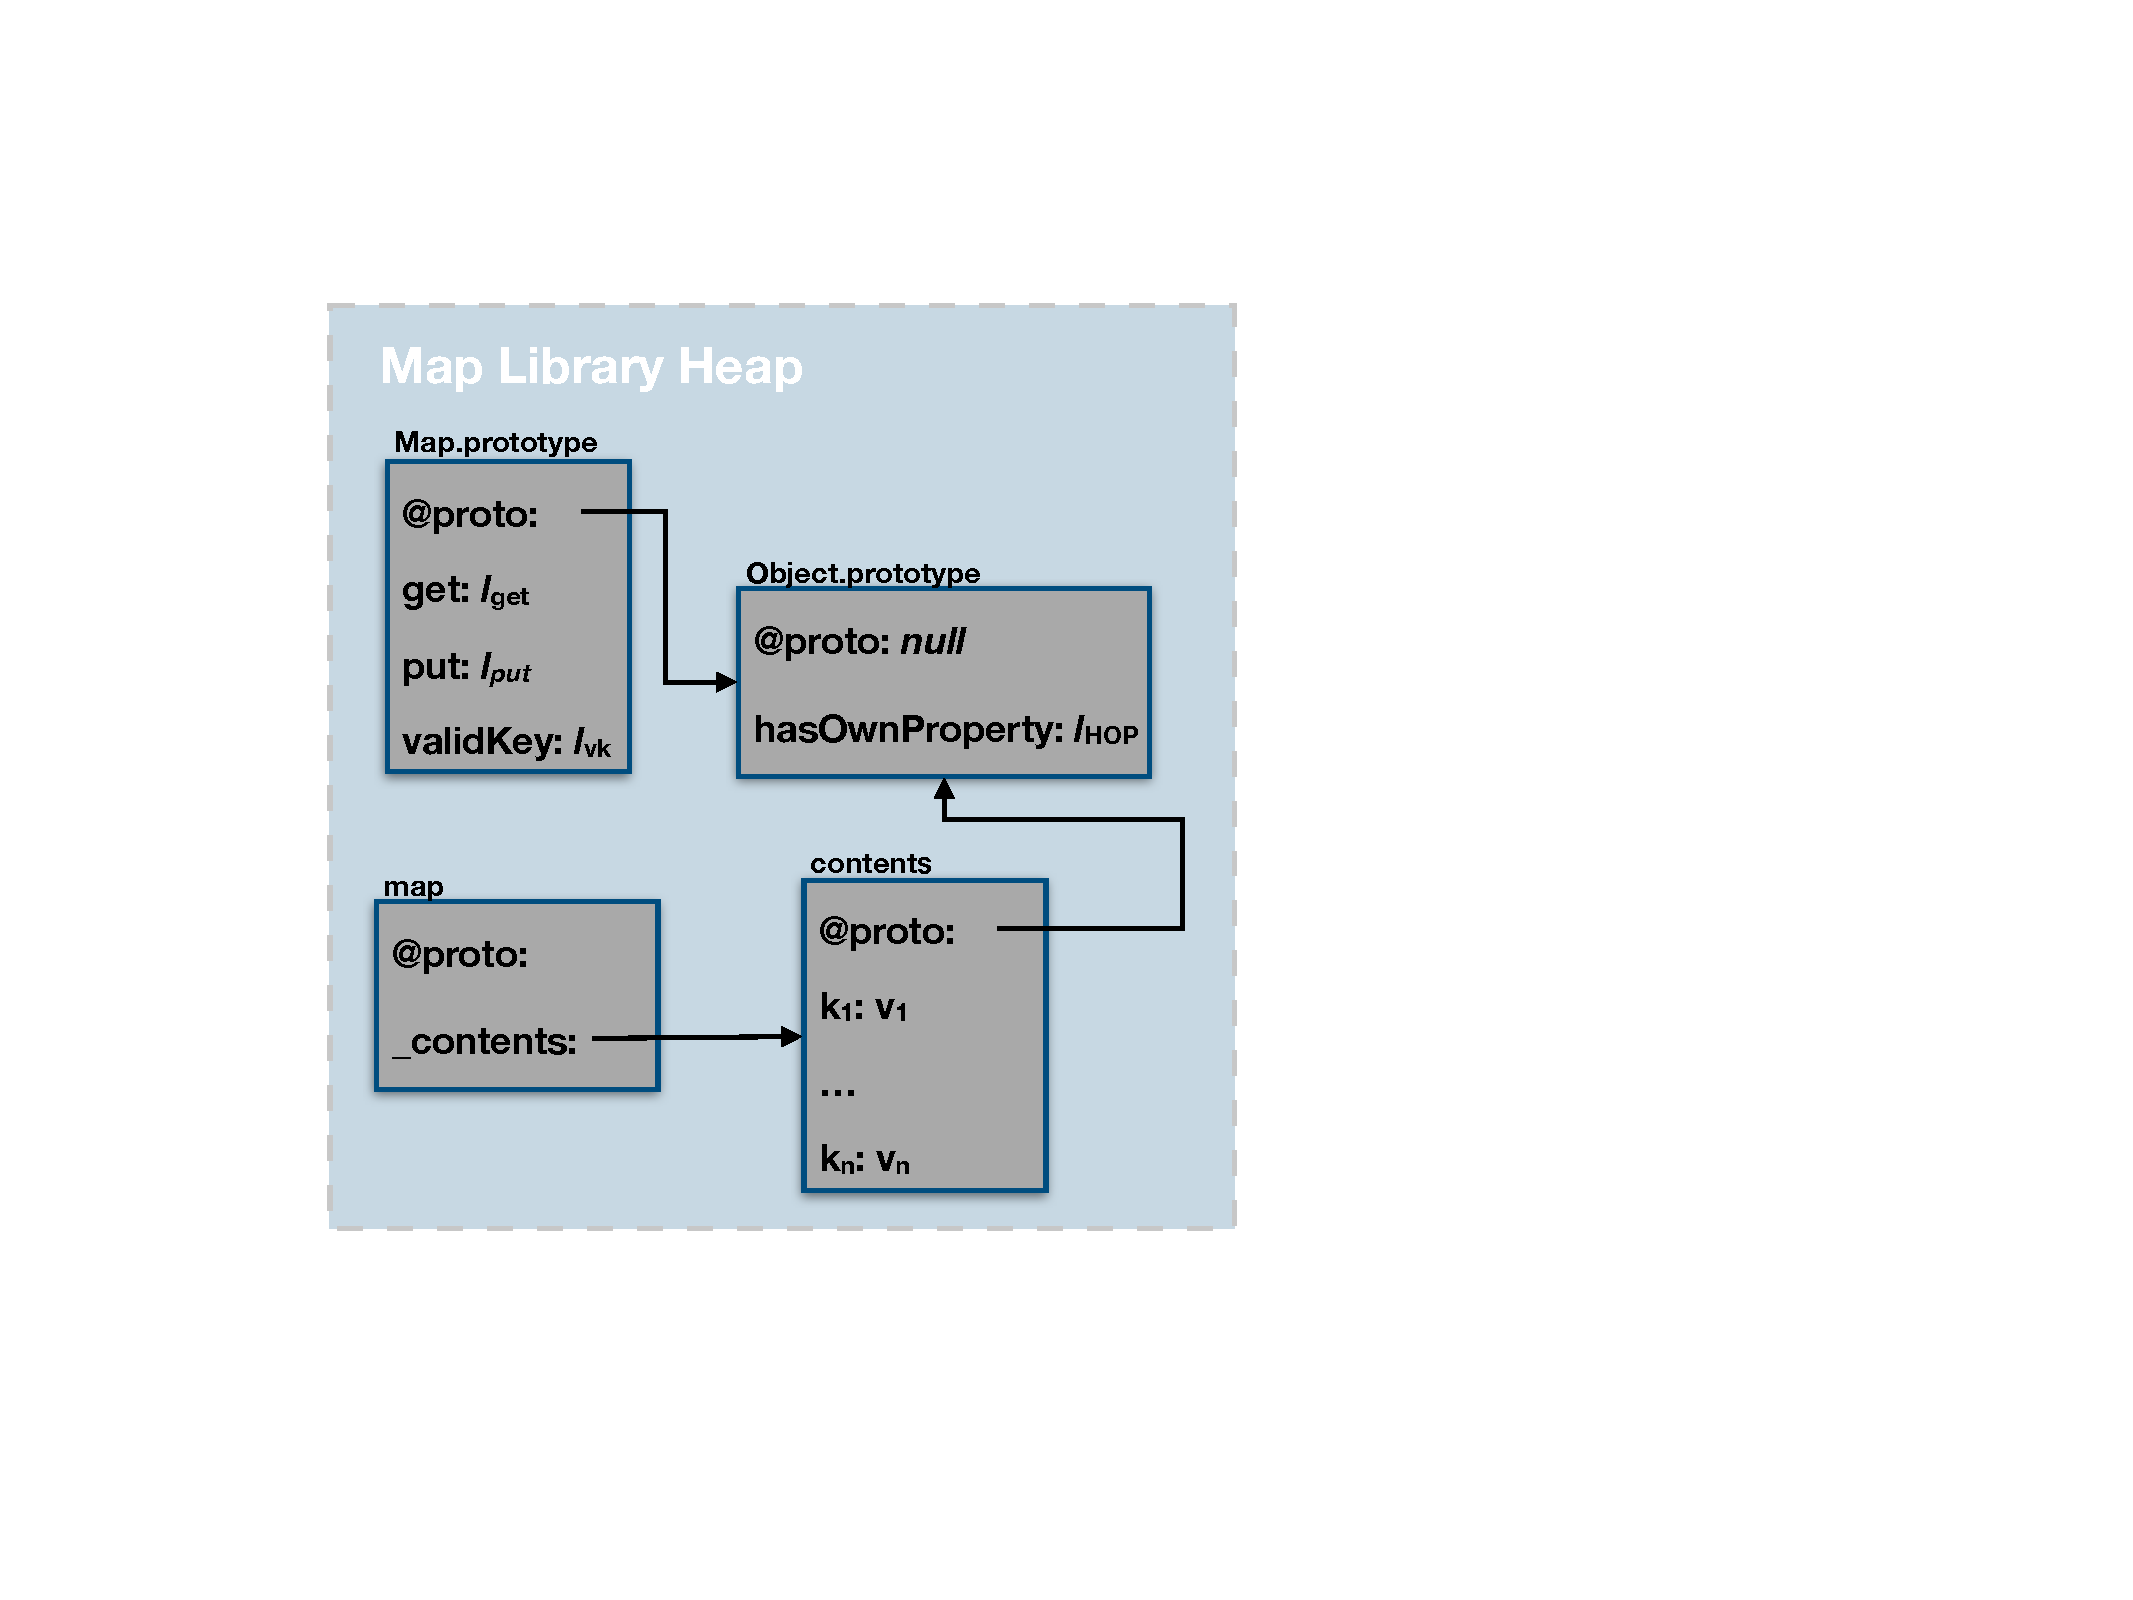
\includegraphics[width=1.1\textwidth]{figures/mapDiagram.pdf}
 \end{minipage}
\caption{JS map implementation (left) and example of a map library heap (right) \label{map:example}}
\end{figure}

The map library implements a \emph{key-value map} as an object with property \jsinline|_contents|, denoting the object used to store the map contents.  
The named properties of \jsinline|_contents| and their value attributes correspond to the map keys and values, respectively.
As the functions \jsinline|get|, \jsinline|put|, and \jsinline|validKey| are to be shared between all map 
objects, they are defined as properties of \jsinline|Map.prototype|, which is the prototype 
of the objects that are created using \jsinline|Map| as a constructor (e.g.~using~\jsinline|new Map()|). 
%
Note that one can insert a key-value pair with \jsinline|"hasOwnProperty"| as a key into the map. 
By doing this, \jsinline|"hasOwnProperty"| in the prototype chain of
\jsinline|_contents| is overridden and subsequent calls to \jsinline|get| will fail. 
Consider the following symbolic test:
%
 \begin{lstjs}[firstnumber=1]
 var s1 = __s(); var n1 = __n(); 
var m = new Map();  m.put (s1, n1); var r = m.get(s1);  
assert(n1 = r)
\end{lstjs}
The symbolic test above reveals the bug. In fact, \jilette outputs 
\jsinline|s1 = "hasOwnProperty"| as a failing model for the symbolic test. 
